%% Part of Stellarium User Guide 0.15+
%% History:
%% 2016-04-17 New chapter.


\chapter{Adding Sky Cultures}
\label{ch:SkyCultures}
\chapterauthor*{Georg Zotti, with additions by Alexander Wolf and Susanne M. Hoffmann}


A \indexterm{sky culture} in Stellarium is the entity that consists of 
\begin{itemize}
\item a set of names for constellations 
\item a description of the role these constellations and other celestial features (clouds, polar lights (aurorae), meteors, comets, \ldots) 
      had or still have for the human culture that used or use these constellations, including some relevant background on the culture.
\item stick figure definitions connecting stars into those constellations
\item (optional) a list of names for individual stars
\item (optional) artwork supporting the stick figures
\item (optional) a description of boundaries or borders between the constellations
\item (optional) names and stick figure definitions of additional figures of lesser importance, termed \indexterm{asterisms}.
\end{itemize}
\noindent The CC-licence that the author of the SC chooses, is valid for the entire set of files, i.e. all texts and images provided.

Stellarium comes with a nice set of sky cultures from all
over the world (see section~\ref{sec:gui:view:starlore}). For ethnographers or
historians of science it may be a worthwhile consideration to
illustrate the sky culture of the people they are studying. It is not
very hard to do so, but depending on your data, may require some
skills in image processing.

Some features regarding translation and multilinguality have evolved
over the years, and not all sky cultures currently included in
Stellarium adhere to the standards described above and in the following
sections. Sky cultures will also see continuous development in the
coming versions. If you add a new sky culture, please adhere to this
description for an optimal result!


In the Stellarium program folder you can see a folder
\file{skycultures}. Let us assume you work on Windows and want to create a
new sky culture, say, \emph{myCulture}.

You can take the \file{inuit} directory as template to start with. Just copy the folder 
\file{C:\textbackslash{}Program Files\textbackslash{}Stellarium\textbackslash{}skycultures\textbackslash{}inuit} to
\file{C:\textbackslash{}Users\textbackslash{}[YOU]\textbackslash{}AppData\textbackslash{}Roaming\textbackslash{}Stellarium\textbackslash{} skycultures\textbackslash{}myculture}

In the folder you see image files for the constellation artwork, and all
other files with various extensions are text files. 


\section{Basic Information}
\label{sec:skycultures:info.ini}


In \file{myculture\textbackslash{}info.ini}, change the entries to 
\begin{configfile}[\scriptsize]
[info]
name=myCulture
author=me
credits=my institute (optional)
boundaries=none
classification=personal
license=CC BY-SA 4.0 International Public License
region=Western Europe
\end{configfile}

\noindent (or what seems best for you). The \texttt{name} is used for the list entry in
the Starlore tab in the View dialog (see \ref{sec:gui:view:starlore}). \texttt{author} should be the actual author(s)' name(s). 
The optional \texttt{credits} \newFeature{0.22.2} can be used to mention other involved parties. 

\subsection{Boundaries}
The option ``boundaries'' is optional and may contain the following values:
\begin{description}
\item[none] --- (default) designates that this culture doesn't have constellation boundaries.
\item[iau] --- use this value for variants of ``modern'' sky cultures to enable use of IAU boundaries.
\item[own] --- used for cultures which have their own set of constellation boundaries.
\end{description}

\subsection{Classification}
The option ``classification'' is also optional. \newFeature{0.19.0} It allows some form of quality control:
\begin{description}
  \item[personal] -- this is a personally developed sky culture which
    is not founded in published historical or ethnological research. Stellarium
    may include it when it is ``pretty enough'' without really
    approving its contents.
  \item[traditional] -- (default value) content represents ``common'' knowledge by
    several members of an ethnic community, and the sky culture has
    been developed by members of such community. Our ``Modern''
    sky culture is a key example: it has evolved for about 2500 years in the ``western'' world,
    and modern astronomers use it.
  \item[ethnographic] -- provided by ethnographic researchers based on
    interviews of indigenous people.
  \item[historical] -- based on historical written sources from a
    (usually short) period of the past.
  \item[single] -- represents a single source like a historical atlas,
    or publications of a single author.
  \item[comparative] -- special-purpose compositions \newFeature{0.21.2} of e.g.\ artwork
    from one and stick figures from another sky culture, and optionally
    asterisms as representations of a third. Or comparison of two
    stick figure sets in constellations and asterisms. These figures
    sometimes will appear not to fit together well. This may be
    intended, to explain and highlight just those differences! The
    description text must clearly explain and identify all sources and
    how these differences should be interpreted.
\end{description}

\subsection{License}
\label{sec:skycultures:licenses}
The option ``license'' \newFeature{0.22.2} is technically optional
(for backward compatibility; it defaults to ``unknown''), but we
highly recommend to define it for your sky culture, and it is
mandatory if you want your sky culture to be distributed with
Stellarium to prevent ``unexpected'' distribution of your content to other
software or applications out of our hands.  The license info will be decoded for human
readable hints about allowed permissions for sky culture in the GUI.

We recommend to use one of the following possible licenses in this section: 
\begin{description}
  \item[GNU GPL v2.0 (or later)] -- this is the most famous ``copyleft'' license for code and it may be acceptable also for text and data.
  \item[CC0] (No Rights Reserved) -- this is a ``don't care'' license. Content may be freely distributed without attribution for all purposes. 
  \item[CC BY] (Creative Commons Attribution License) -- this license lets others distribute, remix, adapt, and build upon your work, even commercially, 
    as long as they credit you for the original creation.
    This is the most accommodating of licenses offered. Recommended for maximum dissemination and use of licensed materials.
  \item[CC BY-SA] (Creative Commons Attribution-ShareAlike License) -- this license lets others remix, adapt, and build upon your work even for commercial purposes, 
    as long as they credit you and license their new creations under the identical terms.
    This license is often compared to ``copyleft'' free and open source software licenses. 
	All new works based on yours will carry the same license, so any derivatives will also allow commercial use.
    This is the license used by Wikipedia, and is recommended for materials that would benefit from incorporating content from Wikipedia and similarly licensed projects.
  \item[CC BY-ND] (Creative Commons Attribution-NoDerivatives License) -- this license lets others reuse the work for any purpose, including commercially; 
    however, it cannot be shared with others in adapted form, and credit must be provided to you.
  \item[CC BY-NC] (Creative Commons Attribution-NonCommercial License) -- this license lets others remix, adapt, and build upon your work non-commercially, 
    and although their new works must also acknowledge you and be non-commercial, they don’t have to license their derivative works on the same terms.
  \item[CC BY-NC-SA] (Creative Commons Attribution-NonCommercial-ShareAlike License) -- this license lets others remix, adapt, and build upon your work non-commercially, 
    as long as they credit you and license their new creations under the identical terms.
  \item[CC BY-NC-ND] (Creative Commons Attribution-NonCommercial-NoDerivatives License) -- this license is the most restrictive of the six main Creative Commons licenses, 
    only allowing others to download your works and share them with others as long as they credit you, but they can’t change them in any way or use them commercially.
  \item[FAL] For illustrations we also expect usage of the \textbf{Free Art License}\footnote{\url{https://artlibre.org/licence/lal/en/}} (in addition to any other licenses) --
    it is a ``copyleft'' license that grants the right to freely copy, distribute, and transform creative works. You can specify, e.g., ``GPL2, FAL'' to 
	indicate that the images are additionally released under Free Art License.
\end{description}

\noindent Creative Commons provides a range of licenses\footnote{Creative
  Commons License Chooser --
  \url{https://creativecommons.org/choose/}}, each of which grants
different rights to use the materials licensed under them. All of
these licenses offer more permissions than ``all rights
reserved''. Some of Creative Commons are free and some are
non-free. For example you can apply only the most permissive of its
licenses (\textbf{CC0}, \textbf{CC BY} and \textbf{CC BY-SA}) to
material you create, to meets the Freedom Defined definition of a
``Free Cultural Work''.\footnote{See Creative Commons website to
  details --
  \url{https://creativecommons.org/share-your-work/public-domain/freeworks}}

If you have used one of the keys above in your \texttt{license} entry,
a short (unofficial!  Informative only) description of license
conditions will be displayed. You can use other licenses as well, but
please describe the conditions sufficiently well in a dedicated
\texttt{h2} section close to the end of your
\file{description.en.utf8}.

\paragraph{Caution for users!} While Stellarium is provided under the free GPL v2.0 licence which allows for commercial use,
some of our sky cultures have been contributed under CC NC/ND licenses,
i.e., are for noncommercial use only.  Please respect their heritage
holders and check-out the CC licence version in the description before
you use sky cultures in public events like TV documentaries, YouTube
videos, lectures, planetarium shows or printed matter. If in doubt,
contact the respective authors.

\subsection{Region}
\label{sec:skycultures:region}
The option ``region'' is also optional and marks the origin region of the respective sky culture. \newFeature{1.2}
It allows some form of additional grouping. The names of regions are following the United Nations
geoscheme UN~M49\footnote{Standard country or area codes for statistical use (M49) -- \url{https://unstats.un.org/unsd/methodology/m49/}}:
\begin{description}
	\item[Northern Africa] -- Algeria, Egypt, Libya, Morocco, Sudan, Tunisia, Western Sahara.
	\item[Eastern Africa] -- British Indian Ocean Territory, Burundi, Comoros, Djibouti, Eritrea, Ethiopia, French Southern Territories, Kenya,
          Madagascar, Malawi, Mauritius, Mayotte, Mozambique, Réunion, Rwanda, Seychelles, Somalia, South Sudan, Uganda, United Republic of Tanzania, Zambia, Zimbabwe.
	\item[Central Africa] -- Angola, Cameroon, Central African Republic, Chad, Congo, Democratic Republic of the Congo, Equatorial Guinea, Gabon, Sao Tome and Principe.
	\item[Southern Africa] -- Botswana, Eswatini, Lesotho, Namibia, South Africa.
	\item[Western Africa] -- Benin, Burkina Faso, Cabo Verde, Côte d’Ivoire, Gambia, Ghana, Guinea, Guinea-Bissau, Liberia,
          Mali, Mauritania, Niger, Nigeria, Saint Helena, Senegal, Sierra Leone, Togo.
	\item[Caribbean] -- Anguilla, Antigua and Barbuda, Aruba, Bahamas, Barbados, Bonaire, Sint Eustatius and Saba, British Virgin Islands,
          Cayman Islands, Cuba, Curaçao, Dominica, Dominican Republic, Grenada, Guadeloupe, Haiti, Jamaica, Martinique, Montserrat, Puerto Rico, Saint Barthélemy,
          Saint Kitts and Nevis, Saint Lucia, Saint Martin (French Part), Saint Vincent and the Grenadines, Sint Maarten (Dutch part),
          Trinidad and Tobago, Turks and Caicos Islands, United States Virgin Islands.
	\item[Central America] -- Belize, Costa Rica, El Salvador, Guatemala, Honduras, Mexico, Nicaragua, Panama.
	\item[Southern America] -- Argentina, Bolivia (Plurinational State of), Bouvet Island, Brazil, Chile, Colombia, Ecuador,
          Falkland Islands (Malvinas), French Guiana, Guyana, Paraguay, Peru, South Georgia and the South Sandwich Islands, Suriname,
          Uruguay, Venezuela (Bolivarian Republic of).
	\item[Northern America] -- Bermuda, Canada, Greenland, Saint Pierre and Miquelon, United States of America.
	\item[Antarctica] -- Antarctica.
	\item[Northern Asia] -- Russian Federation (Asian part).
	\item[Central Asia] -- Kazakhstan, Kyrgyzstan, Tajikistan, Turkmenistan, Uzbekistan.
	\item[Eastern Asia] -- China, Hong Kong Special Administrative Region of China, Macao Special Administrative Region of China,
          Democratic People's Republic of Korea, Japan, Mongolia, Republic of Korea, Taiwan.
	\item[South-eastern Asia] -- Brunei Darussalam, Cambodia, Indonesia, Lao People's Democratic Republic, Malaysia, Myanmar,
          Philippines, Singapore, Thailand, Timor-Leste, Viet Nam.
	\item[Southern Asia] -- Afghanistan, Bangladesh, Bhutan, India, Iran (Islamic Republic of), Maldives, Nepal, Pakistan, Sri Lanka.
	\item[Western Asia] -- Armenia, Azerbaijan, Bahrain, Cyprus, Georgia, Iraq, Israel, Jordan, Kuwait, Lebanon, Oman, Qatar,
          Saudi Arabia, State of Palestine, Syrian Arab Republic, Türkiye, United Arab Emirates, Yemen.
	\item[Eastern Europe] -- Belarus, Bulgaria, Czechia, Hungary, Poland, Republic of Moldova, Romania, Russian Federation (European part), Slovakia, Ukraine.
	\item[Northern Europe] -- Åland Islands, Channel Islands, Denmark, Estonia, Faroe Islands, Finland, Iceland, Ireland, Isle of Man, Latvia, Lithuania,
          Norway, Svalbard and Jan Mayen Islands, Sweden, United Kingdom of Great Britain and Northern Ireland.
	\item[Southern Europe] -- Albania, Andorra, Bosnia and Herzegovina, Croatia, Gibraltar, Greece, Holy See, Italy, Malta, Montenegro, North Macedonia, Portugal, San Marino, Serbia, Slovenia, Spain.
	\item[Western Europe] -- Austria, Belgium, France, Germany, Liechtenstein, Luxembourg, Monaco, Netherlands, Switzerland.
	\item[Australasia] -- Australia, Christmas Island, Cocos (Keeling) Islands, Heard Island and McDonald Islands, New Zealand, Norfolk Island.
	\item[Melanesia] -- Fiji, New Caledonia, Papua New Guinea, Solomon Islands, Vanuatu.
	\item[Micronesia] -- Guam, Kiribati, Marshall Islands, Micronesia (Federated States of), Nauru, Northern Mariana Islands, Palau, United States Minor Outlying Islands.
	\item[Polynesia] -- American Samoa, Cook Islands, French Polynesia, Niue, Pitcairn, Samoa, Tokelau, Tonga, Tuvalu, Wallis and Futuna Islands.
\end{description}

\noindent For ``modern'' sky cultures we use the special region name \textbf{World} to define worldwide applicable data.

\begin{figure}[htbp]
	\centering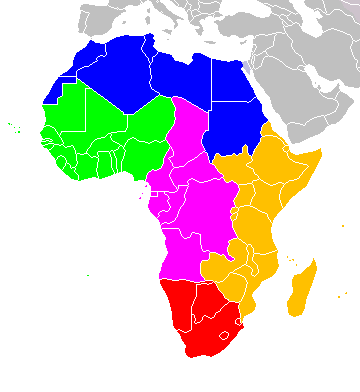
\includegraphics[width=0.75\textwidth]{Africa-regions.png}
	\caption{Africa: subregions as delineated by United Nations geographic classification scheme:
          \ccboxdsc{1.0,0.65,0.0} Eastern Africa, \ccboxdsc{1.0,0.0,1.0} Central Africa, \ccboxdsc{0.0,0.0,1.0} Northern Africa,
          \ccboxdsc{1.0,0.0,0.0} Southern Africa, \ccboxdsc{0.0,1.0,0.0} Western Africa. \emph{Wikipedia / CC BY-SA 3.0}}
	\label{fig:skycultures:AfricaRegions}
\end{figure}

\begin{figure}[htbp]
	\centering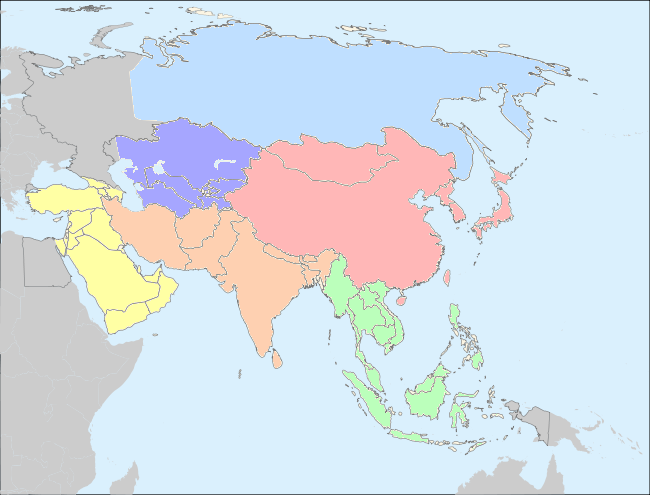
\includegraphics[width=0.75\textwidth]{Asia-regions.png}
	\caption{Asia: subregions as delineated by United Nations geographic classification scheme: \ccboxdsc{0.0,0.0,1.0} Central Asia,
          \ccboxdsc{1.0,0.0,0.0} Eastern Asia, \ccboxdsc{0.0,1.0,0.0} South-eastern Asia, \ccboxdsc{1.0,0.65,0.0} Southern Asia,
          \ccboxdsc{1.0,1.0,0.0} Western Asia, \ccboxdsc{0.75,0.88,1.0} Northern Asia. \emph{Wikipedia / CC BY-SA 3.0}}
	\label{fig:skycultures:AsiaRegions}
\end{figure}

\begin{figure}[htbp]
	\centering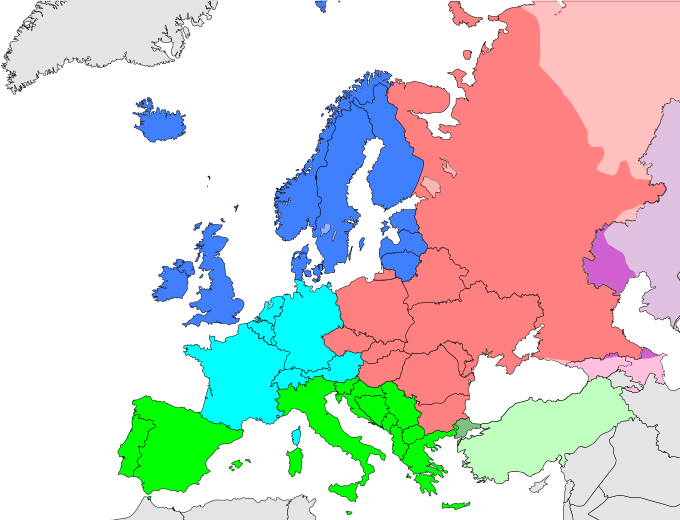
\includegraphics[width=0.75\textwidth]{Europe-regions.png}
	\caption{Europe: subregions as delineated by United Nations geographic classification scheme: \ccboxdsc{1.0,0.5,0.5} Eastern Europe,
          \ccboxdsc{0.25,0.5,1.0} Northern Europe, \ccboxdsc{0.0,1.0,0.0} Southern Europe, \ccboxdsc{0.0,1.0,1.0} Western Europe. \emph{Wikipedia / CC BY-SA 3.0}}
	\label{fig:skycultures:EuropeRegions}
\end{figure}

\begin{figure}[htbp]
	\centering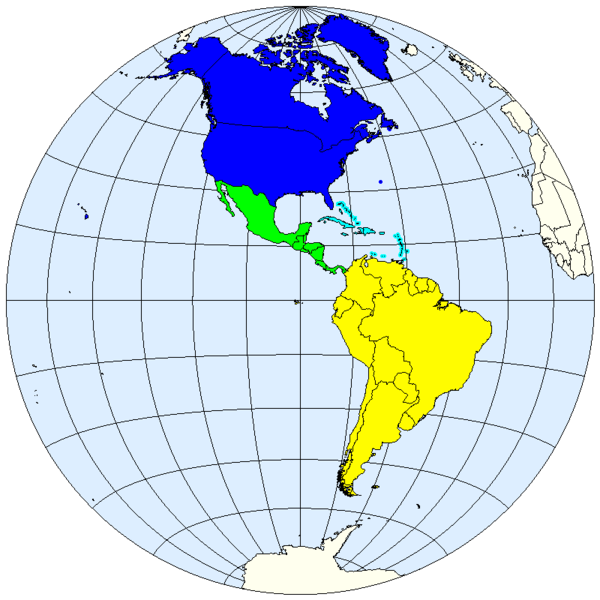
\includegraphics[width=0.7\textwidth]{Americas-regions.png}
	\caption{Americas: subregions as delineated by United Nations geographic classification scheme: \ccboxdsc{0.0,1.0,1.0} Caribbean,
          \ccboxdsc{0.0,1.0,0.0} Central America, \ccboxdsc{0.0,0.0,1.0} Northern America, \ccboxdsc{1.0,1.0,0.0} Southern America. \emph{Wikipedia / CC BY-SA 3.0}}
	\label{fig:skycultures:AmericasRegions}
\end{figure}

\begin{figure}[htbp]
	\centering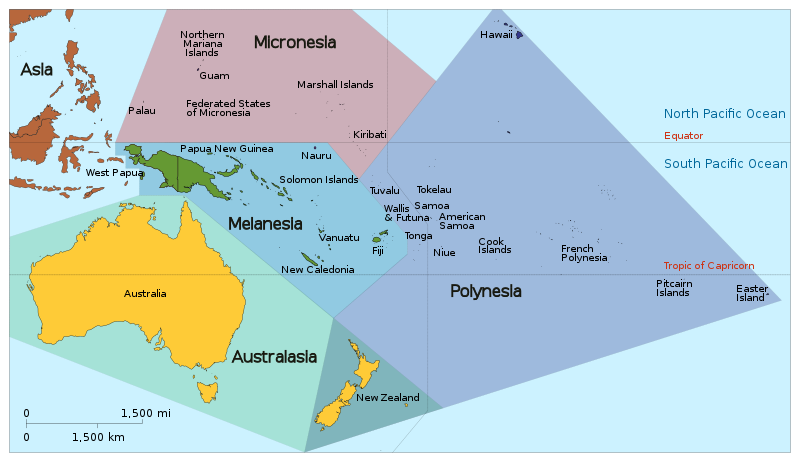
\includegraphics[width=\textwidth]{Oceania-regions.png}
	\caption{Oceania: subregions as delineated by United Nations geographic classification scheme: \ccboxdsc{1.0,0.8,0.2} Australasia, 
          \ccboxdsc{0.6,0.8,0.9} Melanesia, \ccboxdsc{0.8,0.7,0.7} Micronesia, \ccboxdsc{0.62,0.73,0.87} Polynesia. \emph{Wikipedia / CC BY-SA 3.0}}
	\label{fig:skycultures:OceaniaRegions}
\end{figure}

\section{Sky culture Description Files}
\label{sec:skycultures:description}


In order to have translated texts, Stellarium uses files
\file{description.<LANG>.utf8}, where \file{<LANG>} is the two-letter
ISO~639-1 language code, or its extension which contains language and
country code, like \file{pt\_BR} for Brazilian Portuguese. A minimum
sky culture must contain the file \file{description.en.utf8}, this is
\texttt{en=English} text with HTML tags for sections, tables,
etc. You can also have embedded images in the HTML (your book cover?
Views of sacred landscapes/buildings/artwork/\ldots?), just make them
PNG or JPG format please. The length of the description texts is not limited.
You should provide a good description in the interest of future users:
some cultural/ethnographical background of the users of this sky culture,
history of sky culture research that provided this work, tables of names/translations,
links to external resources, whatever seems suitable. When you started
from a copied sky culture, delete the other \file{description.*.utf8}
files.

If you can provide other languages supported by Stellarium, you can
provide translations yourself, else Stellarium translators \emph{may}
translate the English version for you. (It may take years though.) The file
ending \file{.utf8} indicates that for special characters like ÄÖÜßáé
you should use UTF-8 encoding. If you write only English/ASCII, this may not
be relevant.

\section{Proper Names}
\label{sec:skycultures:names}

\subsection{Constellation Names}
\label{sec:skycultures:constellations}

The native constellations are listed in
\file{constellation\_names.eng.fab}. It consists of 3 simple columns:
Abbreviation (or just a serial number), native name, and English
translation. The writing \texttt{\_("name")} allows automatic
translation of the English strings to other languages. These strings
will be used as constellation labels.

You can \newFeature{0.19.2} add a reference comment after each
3-column entry. Just add a white-space, and then a comma-separated list
of numerical references to the books listed in \file{reference.fab}.

The first column (abbreviation) in the Modern sky culture provides
the canonical 3-letter abbreviation for constellations as used by the
International Astronomical Union. Such abbreviations may not be
available for the sky culture you are working with, so you must invent
your own. These abbreviations are used as keys in the other files, so
they must be unique within your sky culture. It is not necessary to have
3-letter keys, but they should act as mnemonic support, so numerical keys are not recommended. 

The keys can be displayed on screen when labels are requested in the
Starlore GUI (section~\ref{sec:gui:view:starlore}). If you want to prevent
certain abbreviations from being displayed, let them start with a
dot. See the effect in the \file{Modern (H.A.Rey)} sky culture: In
\menu{Abbreviated} mode, only the official abbreviations are
displayed. In \menu{Native} mode, the second column of
\file{constellation\_names.eng.fab} is shown. Only with setting
\menu{Translated}, the text translated from the text shown in the
third column is shown. If your sky culture is a variant of the \file{Modern}
sky culture, please use the canonical Latin names, they have all been translated already.

If your sky culture is not a variant of the generally known \file{Modern} (western)
sky culture, please include an English translation to the name given in
the native language. Else translators will not be able to translate
the name. See a good example in the \file{Mongolian} sky culture.

\subsection{Star Names}
\label{sec:skycultures:starnames}

The file \file{star\_names.fab} contains a list of HIP catalog
numbers and common names for those stars. Each line of the file
contains one record of two fields (separated by the pipe character
(\texttt{|})) or three fields (the first pair is separated by the 
pipe character (\texttt{|}) and the last one separated by the space 
character). The first field is the star's Hipparcos catalog number,
the second is the common name of the star in a format that enables
translation support, the third is an optional list of references (see \ref{sec:skycultures:references})  
to the source of the information about this name, e.g:
\begin{configfile}
# Piscis Austrinus (PsA)
113368|_("Fomalhaut") 1,2,6,11,12
113368|_("Thalim")
\end{configfile}

In the sample you can see 3 lines: the first line is a comment, the 
second line has 3 fields and the third line has 2 fields. Both lines 
with data have the same Hipparcos number of the star: \textit{Fomalhaut} is 
the well-known name of HIP 113368, and \textit{Thalim} is an additional 
(not well-known) name of this star for which a source reference is unfortunately missing.

\subsection{Planet Names}
\label{sec:skycultures:planetnames}

The file \file{planet\_names.fab} contains a list of native names of
the planets. Each line of the file contains one record of 3 fields,
separated by the white space or tab character. The first field is the
English name of the planet, the second is the native name of the
planet (can be in the native language, but please for maximum
utability use an English transliteration) and the third is the
translatable version of the native name of the planet (translated into
English). Here is an example from the \file{Egyptian} sky culture:

\begin{configfile}
Mars	"Horus-Desher"	_("Red Horus")
\end{configfile}

\subsection{Deep-Sky Objects Names}
\label{sec:skycultures:dsonames}

\noindent\newFeature{0.15.1}The file \file{dso\_names.fab} contains a list of native names for
deep-sky objects (DSO). The format of this file is similar to the 
\file{star\_names.fab} format (see \ref{sec:skycultures:starnames}).
Each line of the file contains one record of two fields (separated 
by the pipe character (\texttt{|})) or three fields (first pair is 
separated by the pipe character (\texttt{|}) and the last one separated 
by the space character). The first field is an identifier of the
deep-sky object, the second is the native name of the DSO in a 
format that enables translation support, the optional third is a  
list of references (see \ref{sec:skycultures:references}) to the source 
of the information about this name, e.g.:
\begin{configfile}
PGC 17223|_("Native name for LMC") 1,2,3
NGC 292  |_("Native name for SMC") 1,3
NGC 292  |_("Small Magellanic Cloud")
\end{configfile}

\section{Stick Figures}
\label{sec:skycultures:stickfigures}

The modern-style stick figures are coded in \file{constellationship.fab}\footnote{%
  To clarify some apparent misunderstanding of the name: this is not a new word
  coined with -ship as in ``friendship'', but simply constellations encoded in HIPparcos numbers.}.
Lines look like:

\begin{configfile}
Abbr pairs pair1_star1 pair1_star2 pair2_star1 pair2_star2 ...
\end{configfile}
In this file,
\begin{description}
\item[Abbr] is the abbreviation defined in \file{constellation\_names.eng.fab}
\item[pairs] is the number of line pairs which follow.
\item[pairN\_starA] Hipparcos numbers for the stars which form the
  constellation stick figure. We need two entries per line, longer
  line segments are not supported. To find the HIP number, just have
  Stellarium open and click on the star in Stellarium while editing
  this file.
\end{description}
Anything after the last star number is currently ignored.
Comments can be given in lines starting with \texttt{\#} signs. Empty lines are ignored.

\section{Constellation Boundaries}
\label{sec:skycultures:boundaries}

An optional file\footnote{Please define \texttt{boundaries = own} in the file \file{info.ini} to enable using custom boundaries.} 
\file{constellation\_boundaries.dat} can provide data for the boundary lines drawn between constellations. 
The boundaries for the IAU constellations are defined in the file named \file{data/constellation\_boundaries.dat}.
The format for this file is a bit more difficult than the other files. It contains sections which may consist of multiple lines, of the format:

\begin{configfile}
N RA_1 DE_1 RA_2 DE_2 ... RA_N DE_N 2 CON1 CON2
\end{configfile}
where
\begin{description}
\item[N] number of segments for boundary
\item[RA\_n, DE\_n] right ascension (decimal hours) and declination (decimal degrees) of the points of segments in J2000 coordinates.
\item[2 CON1 CON2] this data indicate ``border between 2 constellations CON1 and CON2''. 
      They are used to define isolated boundaries for each constellation (for proper working of the \menu{Select single constellation} option). 
\end{description}

\section{Constellation Artwork}
\label{sec:skycultures:artwork}

Constellation artwork is optional, but may give your sky culture the
final touch, if it requires artwork at all. E.g., H. A. Rey's variant
of the \file{Modern} sky culture deliberately does not contain artwork
other than his new set of stick figures.

Each constellation artwork is linked to 3 stars in its constellation. This
is programmed in the file \file{constellationsart.fab}. It consists of lines

\begin{configfile}
  Abbr image_name.png x1 y1 HIP1 x2 y2 HIP2 x3 y3 HIP3
\end{configfile}
where 
\begin{description}
\item[Abbr] is the abbreviation defined in \file{constellation\_names.eng.fab}
\item[image\_name.png] is the file name of your texture. It should be
  sized in a power of two, like $512\times512$, $1024\times2048$
  etc. Avoid dimensions larger than 2048, they are not supported on
  all systems. Use as little border in your textures as possible instead.
  You can distort images to better exploit the pixels,
  the texture will be stretched back. The background of the artwork
  image must be absolutely black.
\item[x\textit{n}, y\textit{n}, HIP\textit{n}] ($n\in[1, 2, 3]$) pixel locations of the
  star in the constellation drawing (find those in any image editor)
  and HIP\textit{n} is the star number in the Hipparcos catalog, which
  you find when you click on the star in Stellarium.
\end{description}

In case the artwork is only available in a certain projection (e.g.,
an all-sky map), or is otherwise heavily distorted so that the match
is not satisfactory, you may have to re-project the image somehow. For
aligning, you should switch Stellarium to Stereographic projection for
optimal results.

You don't have to shutdown and restart Stellarium during
creation/matching, just switch sky culture to something else and back
to the new one to reload.

\section{Seasonal Rules}
\label{sec:skycultures:seasonal_rules}

File \file{seasonal\_rules.fab} (optional) contains possible seasonal rules for
the visibility of constellations. There is one rule per line. Each
rule contains three elements separated with white space (or tab
character): constellation ID, start of visibility (month) and end of
visibility (month), e.g:

\begin{configfile}
  Emu 6 3
\end{configfile}

\noindent This specifies that constellation Emu (abbreviated also as ``Emu'') is
visible only from June to March.
%% TODO: This feature may need rework. Where is it used?

\section{References}
\label{sec:skycultures:references}

\noindent\newFeature{0.15.1}The file \file{reference.fab} contains a list of information sources. 
Each line of the file contains one record of 3 fields,
separated by the pipe character (\texttt{|}) --- number of source, 
description of source and optional URL, e.g.:

\begin{configfile}
9|Kruger 60|https://en.wikipedia.org/wiki/Kruger_60
\end{configfile}

This file will be used in future versions. It is most important for ``traditional'' 
sky cultures collected from various sources to provide traceable references. 

\section{Asterisms and help rays}
\label{sec:skycultures:asterisms}

\noindent\newFeature{0.16.1}Sometimes there is a need to extract some part of a 
constellation into a figure in its own right, or to merge parts from different 
constellations into one big figure --- e.g. ``Big Dipper'' as part of Ursa Major or the 
``Summer Triangle'' consisting of 3 stars from the constellations Cygnus, Lyra and Aquila. 
After the codification of the official 88 constellations by the IAU, those additional figures
are called \indexterm{asterisms}.\footnote{In a more generalized context when describing the sky of
  other cultures, the distinction may be less strict.}

Other simple figures might be used as navigation helpers: the \indexterm{help rays}. 
As example to help in orientation in the sky the additional lines between constellations 
Ursa Major, Ursa Minor and Cassiopeia might be useful. The asterisms and help rays are listed in
\file{asterism\_names.eng.fab}. This file consists of 2 simple columns:
Abbreviation (or just a serial number) and English
name of asterism. The writing \texttt{\_("name", "asterism")} allows automatic, context sensitive
translation of the English strings to other languages. These strings
will be used as asterisms labels. In addition, after a hash mark (\texttt{\#}) marking a comment sign, 
some reference information can be added in comment lines, like ``List found at \ldots''.
Also, you can \newFeature{0.19.2} again add a reference comment after each
2-column entry. Just add a white-space, and then a comma-separated list
of numerical references to the books listed in \file{reference.fab}.
Collecting sources and giving such references 
is always a good idea. Some later versions of Stellarium may use and display this information.

The stick figures of asterisms are coded in \file{asterism\_lines.fab}
which looks similar to the entries for the constellation
figures. Lines look like:

\begin{configfile}[\scriptsize]
Abbr type pairs pair1_star1 pair1_star2 pair2_star1 pair2_star2 ...
\end{configfile}
or
\begin{configfile}[\scriptsize]
Abbr 2 pairs pair1_RA1 pair1_DE1 pair1_RA2 pair1_DE2 pair2_RA1 ...
\end{configfile}
In this file,
\begin{description}
\item[Abbr] is the abbreviation defined in \file{asterism\_names.eng.fab}
\item[type] is the type of line. Use 1 or 2 to define an asterism and 0 for the help rays (0 and 1 uses HIP numbers, and 2 uses coordinates).
\item[pairs] is the number of line pairs which follow.
\item[pairN\_starA] Hipparcos numbers for the stars which form the asterism/help ray stick figure (similar to constellations),
  or equatorial coordinates for epoch J2000.0 of the stars (decimal hours for right ascension and decimal degrees for declination).
  The help rays are actually a special form of asterisms in Stellarium. 
\end{description}

\section{Publish Your Work}
\label{sec:skyculture:publish}

If you are willing to let other users enjoy the result of your hard
work (and we certainly hope you do!), when you are done, please write
a note in the Forum or at GitHub. We will decide about acceptability
and classification, and may ask for better descriptions for the
benefit of our users.

Please be prepared to put the imagery and text
under some compatible open-source license (Creative Commons).
Else the sky culture cannot be hosted by us.
While we cannot be held responsible for legal problems, it seems that
CC BY 4.0 International\footnote{\url{https://creativecommons.org/licenses/by/4.0/}} or
CC BY-SA 4.0 International\footnote{\url{https://creativecommons.org/licenses/by-sa/4.0/}}
licenses are best suited. See notes in section~\ref{sec:skycultures:licenses} above. 


%%% Local Variables: 
%%% mode: latex
%%% TeX-master: "guide"
%%% End: 

